\documentclass{article}

\usepackage[colorlinks, urlcolor=blue, linkcolor=red, citecolor=green]{hyperref}
\usepackage{fancyhdr} %设置页眉和页脚的
\usepackage{extramarks} %设置continue那玩意的
\usepackage{amsmath}
\usepackage{amsthm}
\usepackage{amsfonts}
\usepackage{tikz} %画线的
\usepackage[plain]{algorithm}
\usepackage{algpseudocode}
\usepackage{enumerate}
\usepackage{color}

\usetikzlibrary{automata,positioning}

%表
\usepackage{booktabs}
\usepackage{multirow}
\usepackage{array}
\usepackage{caption}
\DeclareCaptionFont{heiti}{\heiti} %还可以定义其他的
\captionsetup{labelsep=space, font={small, bf}, skip=2pt} %space可以改成quad

%图
%*****************图片及其相关设置***************************
\usepackage{graphicx}
\graphicspath{{tupian/}}
\usepackage{subfigure}

%*****************代码相关设置***************************
\usepackage{pythonhighlight}
%
% Basic Document Settings
%

\topmargin=-0.45in
\evensidemargin=0in
\oddsidemargin=0in
\textwidth=6.5in
\textheight=9.0in
\headsep=0.25in

\linespread{1.1}

\pagestyle{fancy}
\lhead{\hmwkAuthorName}
\chead{\hmwkClass: \hmwkTitle}
\rhead{\firstxmark}
\lfoot{\lastxmark}
\cfoot{\thepage}

\renewcommand\headrulewidth{0.4pt}
\renewcommand\footrulewidth{0.4pt}

\setlength\parindent{0pt}

%
% Create Problem Sections
%

\newcommand{\enterProblemHeader}[1]{
    \nobreak\extramarks{}{Problem \arabic{#1} continued on next page\ldots}\nobreak{}
    \nobreak\extramarks{Problem \arabic{#1} (continued)}{Problem \arabic{#1} continued on next page\ldots}\nobreak{}
}

\newcommand{\exitProblemHeader}[1]{
    \nobreak\extramarks{Problem \arabic{#1} (continued)}{Problem \arabic{#1} continued on next page\ldots}\nobreak{}
    \stepcounter{#1}
    \nobreak\extramarks{Problem \arabic{#1}}{}\nobreak{}
}

\setcounter{secnumdepth}{0}
\newcounter{partCounter}
\newcounter{homeworkProblemCounter}
\setcounter{homeworkProblemCounter}{1}
\nobreak\extramarks{Problem \arabic{homeworkProblemCounter}}{}\nobreak{}

\newenvironment{homeworkProblem}{
    \section{Problem \arabic{homeworkProblemCounter}}
    \setcounter{partCounter}{1}
    \enterProblemHeader{homeworkProblemCounter}
}{
    \exitProblemHeader{homeworkProblemCounter}
}

%
% Homework Details
%   - Title
%   - Due date
%   - Class
%   - Section/Time
%   - Instructor
%   - Author
%

\newcommand{\hmwkTitle}{Homework\ \#2}
\newcommand{\hmwkDueDate}{April 21, 2021}
\newcommand{\hmwkClass}{Machine Learning}
\newcommand{\hmwkClassTime}{}
\newcommand{\hmwkClassInstructor}{Professor Xiao Li}
\newcommand{\hmwkAuthorName}{Peng Deng}
\newcommand{\hmwkAuthorSchool}{School of Data Science}
\newcommand{\hmwkAuthorNumber}{Sno.220041042}
%
% Title Page
%

\title{
    \vspace{2in}
    \textmd{\textbf{\hmwkClass:\ \hmwkTitle}}\\
    \normalsize\vspace{0.1in}\small{Due\ on\ \hmwkDueDate}\\
    \vspace{0.1in}\large{\textit{\hmwkClassInstructor\ \hmwkClassTime}}
    \vspace{3in}
}

\author{\textbf{\hmwkAuthorName}}

\date{}

\renewcommand{\part}[1]{\textbf{\large Part \Alph{partCounter}}\stepcounter{partCounter}\\}

%
% Various Helper Commands
%

% Useful for algorithms
\newcommand{\alg}[1]{\textsc{\bfseries \footnotesize #1}}
\usepackage[algo2e,vlined,ruled]{algorithm2e}

% For derivatives
\newcommand{\deriv}[1]{\frac{\mathrm{d}}{\mathrm{d}x} (#1)}

% For partial derivatives
\newcommand{\pderiv}[2]{\frac{\partial}{\partial #1} (#2)}

% Integral dx
\newcommand{\dx}{\mathrm{d}x}

% Alias for the Solution section header
\newcommand{\solution}{\textbf{\large Solution}}

% Probability commands: Expectation, Variance, Covariance, Bias
\newcommand{\E}{\mathrm{E}}
\newcommand{\Var}{\mathrm{Var}}
\newcommand{\Cov}{\mathrm{Cov}}
\newcommand{\Bias}{\mathrm{Bias}}
\begin{document}

\maketitle
\thispagestyle{empty}

\newpage
\setcounter{page}{1}

\begin{homeworkProblem}
	Suppose $f$ maps sample space $\mathcal{X}$ to \{0,1\} and let $\mathcal{S}$ be $n$ i.i.d training samples. For any $t>0$, we have the concentration inequality (can be shown by Hoeffding's inequity):
$$
\operatorname{Pr}\left[\left|\operatorname{Er}_{\text {in }}(f)-\operatorname{Er}_{\text {out }}(f)\right|>t\right] \leq 2 e^{-2 n t^{2}}
$$
Show that the variance of $\operatorname{Er}_{\text {in }}(f)$ satisfies $\operatorname{Var}\left[\operatorname{Er}_{\text {in }}(f)\right] \leq \frac{\log (2 e)}{n}$.(\textbf{Hint}: use $\mathbb{E}\left[X^{2}\right]=\int_{0}^{\infty} \operatorname{Pr}\left[X^{2}>\right.$
$t] d t)$
	
\vspace{4pt}
\textbf{\large{Solution}}

\begin{equation}
    \begin{split}
        \operatorname{Var}\left[\operatorname{Er_{in}}\left(f\right)\right] &= \operatorname{E}\left[\left(\operatorname{Er_{in}}\left(f\right)-\operatorname{E}_{\mathcal{S}\sim\mathcal{D}}\left[\operatorname{Er_{in}}\left(f\right)\right]\right)^2\right]\\
        &=\int_0^{\infty}\operatorname{Pr}\left[\left(\operatorname{Er_{in}}\left(f\right)-\operatorname{E}_{\mathcal{S}\sim\mathcal{D}}\left[\operatorname{Er_{in}}\left(f\right)\right]\right)^2>t\right]dt\\
        &=\int_0^{\infty}\operatorname{Pr}\left[\left|\operatorname{Er_{in}}\left(f\right)-\operatorname{E}_{\mathcal{S}\sim\mathcal{D}}\left[\operatorname{Er_{in}}\left(f\right)\right]\right|>\sqrt{t}\right]dt\\
        &\le \int_0^{\infty}2e^{-2nt}dt\\
        &=\frac{1}{n}\\
        &\leq\frac{\log (2 e)}{n}
    \end{split}
\end{equation}
Thus, we finished the proof.
\end{homeworkProblem}
\begin{homeworkProblem}
Suppose $f \in \mathcal{H}$ maps sample space $\mathcal{X}$ to \{0,1\} . The Rademacher complexity bound derived in our lecture is by applying McDiarmid's inequality to
$$
h(\mathcal{S})=\sup _{f \in \mathcal{H}}\left[\operatorname{Er}_{\text {out }}(f)-\operatorname{Er}_{\text {in }}(f)\right]
$$
Try to obtain a generalization bound in terms of the empirical Rademacher complexity $\widehat{\mathcal{R}}_{\mathcal{S}}(\mathcal{H})$ by applying McDiarmid's inequality to
$$
\Psi(\mathcal{S})=\sup _{f \in \mathcal{H}}\left[\mathrm{Er}_{\mathrm{out}}(f)-\operatorname{Er}_{\mathrm{in}}(f)-\widehat{\mathcal{R}}_{\mathcal{S}}(\mathcal{H})\right]
$$
\textbf{Hint}: You can follow the analysis in slides 6 page $20-21$ and use directly the result in slides 6 page $22-24$ that $\mathbb{E}[h(\mathcal{S})] \leq \mathcal{R}(\mathcal{H})$.
	
\vspace{4pt}
\textbf{\large{Solution}}

Firstly, we check the condition in McDiarmid’s inequality. Let 
\begin{equation}\nonumber
    \begin{split}
        \mathcal{S}&=\left\{\boldsymbol{z}_1, \cdots,\textcolor{red}{\boldsymbol{z}_i},\cdots ,\boldsymbol{z}_n \right\}\\
        \mathcal{S}^{\prime}&=\left\{\boldsymbol{z}_1, \cdots,\textcolor{red}{\boldsymbol{z}^{\prime}_i},\cdots ,\boldsymbol{z}_n \right\}
    \end{split}
\end{equation}
We have 
\begin{equation}
    \label{eqx}
    \begin{split}
        \Psi\left(\mathcal{S}^{\prime}\right)-\Psi\left(\mathcal{S}\right)&=\sup _{f \in \mathcal{H}}\left[\mathrm{Er}_{\mathrm{out}}(f)-\operatorname{Er}_{\mathrm{in}}(f;\mathcal{S}^{\prime})-\widehat{\mathcal{R}}_{\mathcal{S}^{\prime}}(\mathcal{H})\right]-\sup _{f \in \mathcal{H}}\left[\mathrm{Er}_{\mathrm{out}}(f)-\operatorname{Er}_{\mathrm{in}}(f;\mathcal{S})-\widehat{\mathcal{R}}_{\mathcal{S}}(\mathcal{H})\right]\\
        &\leq \sup _{f \in \mathcal{H}}\left[\operatorname{Er}_{\mathrm{in}}(f;\mathcal{S})+\widehat{\mathcal{R}}_{\mathcal{S}}(\mathcal{H})-\operatorname{Er}_{\mathrm{in}}(f;\mathcal{S}^{\prime})-\widehat{\mathcal{R}}_{\mathcal{S}^{\prime}}(\mathcal{H})\right]\\
        &=\sup _{f \in \mathcal{H}}\left[\frac{e\left(f\left(\boldsymbol{x}_i\right),y_i\right)-e\left(f\left(\boldsymbol{x}^{\prime}_i\right),y^{\prime}_i\right)}{n}+\widehat{\mathcal{R}}_{\mathcal{S}}(\mathcal{H})-\widehat{\mathcal{R}}_{\mathcal{S}^{\prime}}(\mathcal{H})\right]\\
        &\leq\sup _{f \in \mathcal{H}}\left[\frac{e\left(f\left(\boldsymbol{x}_i\right),y_i\right)-e\left(f\left(\boldsymbol{x}^{\prime}_i\right),y^{\prime}_i\right)}{n}\right] +\sup _{f \in \mathcal{H}}\left[\widehat{\mathcal{R}}_{\mathcal{S}}(\mathcal{H})-\widehat{\mathcal{R}}_{\mathcal{S}^{\prime}}(\mathcal{H})\right]\\
        &=\sup _{f \in \mathcal{H}}\left[\frac{e\left(f\left(\boldsymbol{x}_i\right),y_i\right)-e\left(f\left(\boldsymbol{x}^{\prime}_i\right),y^{\prime}_i\right)}{n}\right] +\widehat{\mathcal{R}}_{\mathcal{S}}(\mathcal{H})-\widehat{\mathcal{R}}_{\mathcal{S}^{\prime}}(\mathcal{H})\\
        &\leq \frac{1}{n} + \widehat{\mathcal{R}}_{\mathcal{S}}(\mathcal{H})-\widehat{\mathcal{R}}_{\mathcal{S}^{\prime}}(\mathcal{H})
    \end{split}
\end{equation}
Then, let's consider $\widehat{\mathcal{R}}_{\mathcal{S}}(\mathcal{H})-\widehat{\mathcal{R}}_{\mathcal{S}^{\prime}}(\mathcal{H})$
\begin{equation}
    \begin{split}
        &\widehat{\mathcal{R}}_{\mathcal{S}}(\mathcal{H})-\widehat{\mathcal{R}}_{\mathcal{S}^{\prime}}(\mathcal{H})\\
        &=\mathrm{E}_{\boldsymbol{\epsilon}}\left[\sup _{f \in \mathcal{H}} \frac{1}{n} \left[\epsilon_{1} f\left(\boldsymbol{x}_{1}\right)+\cdots + \epsilon_{i} f\left(\boldsymbol{x}_{i}\right)+\cdots+\epsilon_{n} f\left(\boldsymbol{x}_{n}\right)\right]\right]-\mathrm{E}_{\boldsymbol{\epsilon}}\left[\sup _{f \in \mathcal{H}} \frac{1}{n} \left[\epsilon_{1} f\left(\boldsymbol{x}_{1}\right)+\cdots + \epsilon_{i} f\left(\boldsymbol{x}^{\prime}_{i}\right)+\cdots+\epsilon_{n} f\left(\boldsymbol{x}_{n}\right)\right]\right]\\
        &=\mathrm{E}_{\boldsymbol{\epsilon}}\left[\sup _{f \in \mathcal{H}} \frac{1}{n} \left[\epsilon_{1} f\left(\boldsymbol{x}_{1}\right)+\cdots + \epsilon_{i} f\left(\boldsymbol{x}_{i}\right)+\cdots+\epsilon_{n} f\left(\boldsymbol{x}_{n}\right)\right]-\sup _{f \in \mathcal{H}} \frac{1}{n} \left[\epsilon_{1} f\left(\boldsymbol{x}_{1}\right)+\cdots + \epsilon_{i} f\left(\boldsymbol{x}^{\prime}_{i}\right)+\cdots+\epsilon_{n} f\left(\boldsymbol{x}_{n}\right)\right]\right]\\
        &\leq\mathrm{E}_{\boldsymbol{\epsilon}}\left[\sup _{f \in \mathcal{H}}\frac{\epsilon_{i}}{n}\left[ f\left(\boldsymbol{x}_{i}\right)- f\left(\boldsymbol{x}^{\prime}_{i}\right)\right]\right]\\
        &=\left[\sup _{f \in \mathcal{H}}\frac{1}{n}\left[ f\left(\boldsymbol{x}_{i}\right)-f\left(\boldsymbol{x}^{\prime}_{i}\right)\right]\right]\cdot \frac{1}{2} + \left[\sup _{f \in \mathcal{H}}\frac{-1}{n}\left[ f\left(\boldsymbol{x}_{i}\right)-f\left(\boldsymbol{x}^{\prime}_{i}\right)\right]\right]\cdot \frac{1}{2}\\
        &\leq\frac{1}{2n} + \frac{1}{2n}\\
        &=\frac{1}{n}
    \end{split}
\end{equation}
Back to equation (\ref{eqx}), we have 
\begin{equation}
    \begin{split}
        \Psi\left(\mathcal{S}^{\prime}\right)-\Psi\left(\mathcal{S}\right)&\leq \frac{1}{n} + \widehat{\mathcal{R}}_{\mathcal{S}}(\mathcal{H})-\widehat{\mathcal{R}}_{\mathcal{S}^{\prime}}(\mathcal{H})\\
        &\leq \frac{1}{n} + \frac{1}{n}\\
        &=\frac{2}{n}
    \end{split}
\end{equation}
Due to symmetric, we also have 
\begin{equation}
    \begin{split}
        \Psi\left(\mathcal{S}\right)-\Psi\left(\mathcal{S}^{\prime}\right)&\leq\frac{2}{n}
    \end{split}
\end{equation}
Thus, we have 
\begin{equation}
    \left|\Psi\left(\mathcal{S}\right)-\Psi\left(\mathcal{S}^{\prime}\right)\right|\leq \frac{2}{n}
\end{equation}
Thus, the condition in McDiarmid’s inequality is satisfied. Apply McDiarmid’s inequality to $\Psi\left(\mathcal{S}\right)$, we have
\begin{equation}
    \begin{split}
        \operatorname{Pr}\left[\Psi\left(\mathcal{S}\right)-\operatorname{E}\left[\Psi\left(\mathcal{S}\right)\right]\geq t\right]\leq e^{\frac{-nt^2}{2}}, \quad\forall t > 0 
    \end{split}
\end{equation}
Let $\delta=e^{\frac{-nt^2}{2}}$, we then have with probability at least 1-$\delta$
\begin{equation}
    \label{eq1-8}
    \Psi\left(\mathcal{S}\right)\leq \operatorname{E}\left[\Psi\left(\mathcal{S}\right)\right]+\sqrt{\frac{2\log\left(\frac{1}{\delta}\right)}{n}}
\end{equation}
Since
\begin{equation}
    \label{eq1-9}
    \begin{split}
        \Psi(\mathcal{S})=\sup _{f \in \mathcal{H}}\left[\mathrm{Er}_{\mathrm{out}}(f)-\operatorname{Er}_{\mathrm{in}}(f)-\widehat{\mathcal{R}}_{\mathcal{S}}(\mathcal{H})\right]\geq \mathrm{Er}_{\mathrm{out}}(f)-\operatorname{Er}_{\mathrm{in}}(f)-\widehat{\mathcal{R}}_{\mathcal{S}}(\mathcal{H}), \quad \forall f\in\mathcal{H}
    \end{split}
\end{equation}

By combining equation (\ref{eq1-8}) and (\ref{eq1-9}), we obtain
\begin{equation}
    \label{eq1-10}
    \begin{split}
        \forall f\in \mathcal{H}, \quad \mathrm{Er}_{\mathrm{out}}(f)&\leq \operatorname{Er}_{\mathrm{in}}(f)+\widehat{\mathcal{R}}_{\mathcal{S}}(\mathcal{H})+\Psi(\mathcal{S})\\
        &\leq\operatorname{Er}_{\mathrm{in}}(f)+\widehat{\mathcal{R}}_{\mathcal{S}}(\mathcal{H})+\operatorname{E}\left[\Psi\left(\mathcal{S}\right)\right]+\sqrt{\frac{2\log\left(\frac{1}{\delta}\right)}{n}}\\
    \end{split}
\end{equation}
Then, we consider the term $\operatorname{E}\left[\Psi\left(\mathcal{S}\right)\right]$ as follow
\begin{equation}
    \label{eq1-11}
    \begin{split}
        \operatorname{E}\left[\Psi\left(\mathcal{S}\right)\right] &= \operatorname{E}_{\mathcal{S}\sim i.i.d.\mathcal{D}}\left[ \sup _{f \in \mathcal{H}}\left[\mathrm{Er}_{\mathrm{out}}(f)-\operatorname{Er}_{\mathrm{in}}(f)-\widehat{\mathcal{R}}_{\mathcal{S}}(\mathcal{H})\right]\right]\\
        &=\operatorname{E}_{\mathcal{S}}\left[\sup _{f \in \mathcal{H}}\left[\mathrm{Er}_{\mathrm{out}}(f)-\operatorname{Er}_{\mathrm{in}}(f)\right]-\widehat{\mathcal{R}}_{\mathcal{S}}(\mathcal{H})\right]\\
        &=\operatorname{E}_{\mathcal{S}}\left[h\left(\mathcal{S}\right)-\widehat{\mathcal{R}}_{\mathcal{S}}(\mathcal{H})\right]\\
        &=\operatorname{E}_{\mathcal{S}}\left[h\left(\mathcal{S}\right)\right]-\operatorname{E}_{\mathcal{S}}\left[\widehat{\mathcal{R}}_{\mathcal{S}}(\mathcal{H})\right]\\
        &\leq \mathcal{R}\left(\mathcal{H}\right)-\mathcal{R}\left(\mathcal{H}\right)\\
        &=0
    \end{split}
\end{equation}
By combining equation \ref{eq1-10} and \ref{eq1-11}, we have 
\begin{equation}
    \begin{split}
        \forall f\in \mathcal{H}, \quad \mathrm{Er}_{\mathrm{out}}(f)&\leq\operatorname{Er}_{\mathrm{in}}(f)+\widehat{\mathcal{R}}_{\mathcal{S}}(\mathcal{H})+\operatorname{E}\left[\Psi\left(\mathcal{S}\right)\right]+\sqrt{\frac{2\log\left(\frac{1}{\delta}\right)}{n}}\\
        &\leq \operatorname{Er}_{\mathrm{in}}(f)+\widehat{\mathcal{R}}_{\mathcal{S}}(\mathcal{H})+\sqrt{\frac{2\log\left(\frac{1}{\delta}\right)}{n}}\\
    \end{split}
\end{equation}
Above all, we obtain the generalization bound in terms of the empirical Rademacher complexity $\widehat{\mathcal{R}}_{\mathcal{S}}(\mathcal{H})$. For any $\delta > 0$, with probability at least $1-\delta$, we have the following generalization bound:
\begin{equation}
    \begin{split}
        \forall f\in \mathcal{H}, \quad \mathrm{Er}_{\mathrm{out}}(f)&\leq \operatorname{Er}_{\mathrm{in}}(f)+\widehat{\mathcal{R}}_{\mathcal{S}}(\mathcal{H})+\sqrt{\frac{2\log\left(\frac{1}{\delta}\right)}{n}}\\
    \end{split}
\end{equation}
\end{homeworkProblem}

\begin{homeworkProblem}
Toy polynomial regression using $\ell_{2}$ -regularization and cross-validation. 

Suppose that we have the underlying model
\begin{equation}
    \label{eq1}
    y=x^{2}+\varepsilon
\end{equation}

We collect $n=10$ data points $\left\{\left(x_{i}, y_{i}\right)\right\}_{i=1}^{n} ;$ see the visualization in Figure \ref{p1}. You can download the data from blackboard.
Now, suppose we are going to fit all the data using 8 -th order polynomials:
\begin{equation}
    \label{eq2}
    y=\theta_{0}+\theta_{1} x+\theta_{2} x^{2}+\theta_{3} x^{3}+\ldots+\theta_{8} x^{8} .
\end{equation}
\begin{figure}[H]
    \centering
    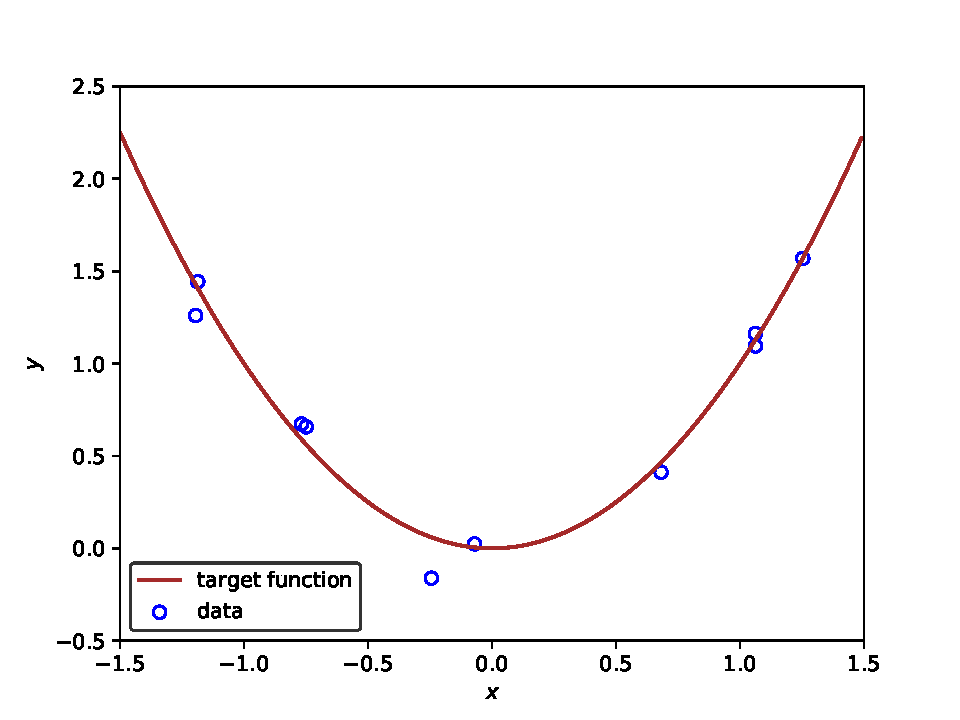
\includegraphics[width=0.5\linewidth]{tupian/original.pdf}
    \caption{Visualization of data}
    \label{p1}
\end{figure}

\begin{description}
    \item [(a1)]Denote the $\boldsymbol{\theta}=\left(\theta_{0}, \ldots, \theta_{8}\right) \in \mathbb{R}^{9}$ as the parameter. We have the following linear model
    $$
    \boldsymbol{y}=\boldsymbol{X} \boldsymbol{\theta}
    $$
    Specify $\boldsymbol{y}$ and $\boldsymbol{X}$ using the training data $\left\{\left(x_{i}, y_{i}\right)\right\}_{i=1}^{n}$
    \item [(a2)]Furthermore, we can formulate the following least squares
    \begin{equation}
        \label{eq3}
        \widehat{\boldsymbol{\theta}}=\underset{\boldsymbol{\theta} \in \mathbb{R}^{9}}{\operatorname{argmin}}\|\boldsymbol{X} \boldsymbol{\theta}-\boldsymbol{y}\|_{2}^{2}
    \end{equation}
    Calculate $\widehat{\boldsymbol{\theta}}$ defined in (\ref{eq3}) and plot the fitted curve in Figure \ref{p1} (limit $x$ -axis from -1.5 to 1.5 and limit $y$ -axis from -0.5 to 2.5 ). You can download the code used to generate Figure \ref{p1} from blackboard.
    \item [(a3)]Using the test data set, calculate the test error $\|\boldsymbol{X}_{\text {test}} \widehat{\boldsymbol{\theta}}-\boldsymbol{y}_{\text {test}}\|_{2}$ of $\widehat{\boldsymbol{\theta}}$ defined in
    (\ref{eq3}).
    \item [(b1)]Since we know that the underlying model in (\ref{eq1}) is quadratic, while the fitting model in (\ref{eq2}) is polynomial of order $8,$ we must have overfitting, which you can see from question (a2) and (a3). One way to prevent overfitting is regularization. Instead of using (\ref{eq3}), we formulate the following $\ell_{2}$ -regularized least squares
    \begin{equation}
        \label{eq4}
        \widehat{\boldsymbol{\theta}}=\underset{\boldsymbol{\theta} \in \mathbb{R}^{9}}{\operatorname{argmin}}\|\boldsymbol{X} \boldsymbol{\theta}-\boldsymbol{y}\|_{2}^{2}+\lambda\|\boldsymbol{\theta}\|_{2}^{2}
    \end{equation}
    However, one difficulty to implementing (\ref{eq4}) is determining the regularization parameter $\lambda$. A too large $\lambda$ leads to underfitting, while a too small $\lambda($ e.g. $\lambda=0)$ results in overfitting. Suppose we set the set of candidates of $\lambda$ as
    \begin{equation}\nonumber
        \left[10^{-5}\quad 10^{-4}\quad10^{-3}\quad 10^{-2}\quad 10^{-1}\quad 0.3\quad 0.5 \quad0.8\quad1\quad2\quad5\quad 10\quad15\quad20\quad50\quad100\right]
    \end{equation}
    using \textbf{5 -fold cross-validation} to select the regularization parameter $\lambda$, and plot the validation error versus the value of $\lambda$, where error is the $y$ -axis and $\lambda$ is the $x$ -axis (set the $x$ -axis to log-scale).

    \item [(b2)]Based on the result in (b1), set $\lambda=0.01,0.1,0.8,$ and 5 in (\ref{eq4}) and solve for the corresponding $\widehat{\boldsymbol{\theta}},$ respectively. Plot the fitted curve using the former four choices of $\lambda$ in Figure \ref{p1} , you have to draw four figures separately (limit $x$ -axis from - 1.5 to 1.5 and limit $y$ -axis from -0.5 to 2.5$)$.
    \item [(b3)]Using the test data set, calculate the test error $\|\boldsymbol{X}_{\text {test}} \widehat{\boldsymbol{\theta}}-\boldsymbol{y}_{\text {test}}\|_{2}$ of each of $\widehat{\boldsymbol{\theta}}$ obtained in (b2).
\end{description}
	
\vspace{4pt}
\textbf{\large{Solution}}
	
\vspace{4pt}
\textbf{Subproblem (a1)}

We can specify $\boldsymbol{y}$ and $\boldsymbol{X}$ as follow.
\begin{equation}
    \begin{split}
        \boldsymbol{y} &= 
        \begin{pmatrix}
            y_1 & y_2 &\cdots &y_n
        \end{pmatrix}^{\top}\\
        \boldsymbol{X} &=
        \begin{pmatrix}
            1&x_1&x_1^2&\cdots&x_1^8\\
            1&x_2&x_2^2&\cdots&x_2^8\\
            \vdots&\vdots&\vdots&\ddots&\vdots\\
            1&x_n&x_n^2&\cdots&x_n^8
        \end{pmatrix}
    \end{split}
\end{equation}
	
\vspace{4pt}
\textbf{Subproblem (a2)}

According to the closed form solution of least squares, we have
\begin{equation}
    \begin{split}
        \boldsymbol{\widehat{\theta}}=\left(\boldsymbol{X}^\top\boldsymbol{X}\right)^{-1}\boldsymbol{X}^{\top}\boldsymbol{y}\\
    \end{split}
\end{equation}
Then, we can plot the fitted curve as Figure \ref{fitted}.
\begin{figure}[H]
    \centering
    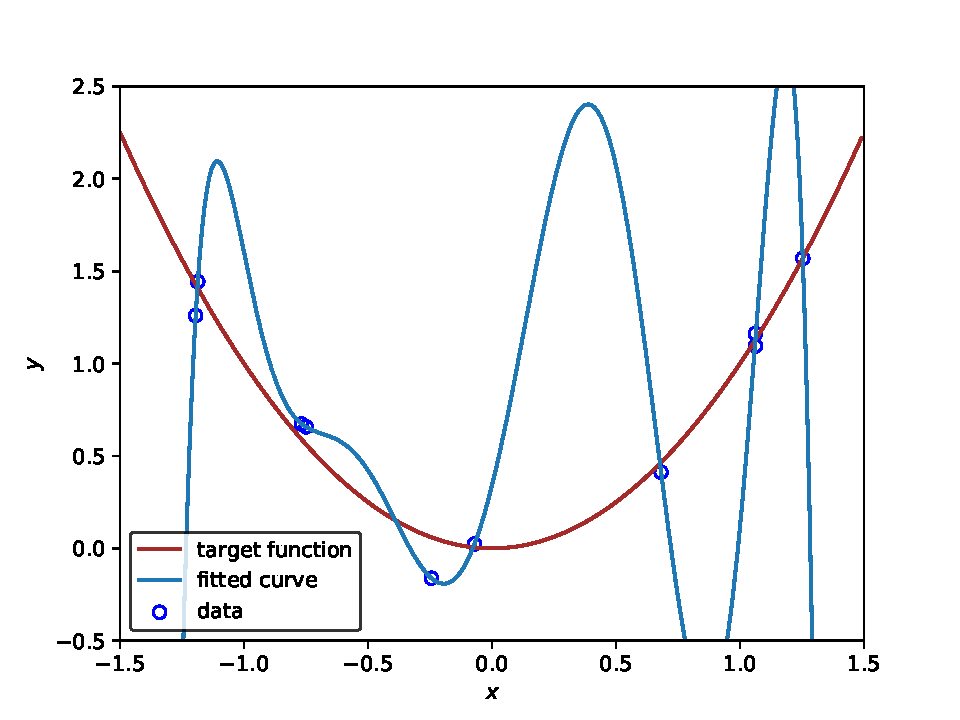
\includegraphics[width=0.5\linewidth]{tupian/fitted.pdf}
    \caption{Fitted curve}
    \label{fitted}
\end{figure}
As we can see from Figure \ref{fitted}, when we use 8-th order polynomials, we can almost fit all the 10 points. However, the fitted curve is far away from the target 
function, which means it is overfitted. Although the in-sample error is small (fit the training data very well), the out of sample error is large, which means the model's generalization ability is not good.
	
\vspace{4pt}
\textbf{Subproblem (a3)}

By using Python, we can compute the test error as follow:
\begin{equation}
    \label{eq6}
    \|\boldsymbol{X}_{\text {test}} \widehat{\boldsymbol{\theta}}-\boldsymbol{y}_{\text {test}}\|_{2} = 106.40
\end{equation}
As we can see from equation \ref{eq6}, the test error is very large, which means the 8-th order polynomial model is overfitted.
	
\vspace{4pt}
\textbf{Subproblem (b1)}

We know that the $\ell_{2}$-regularized least squares has the closed form solution as follow:
\begin{equation}
    \boldsymbol{\widehat{\theta}}=\left(\boldsymbol{X}^\top\boldsymbol{X}+\lambda\boldsymbol{I}\right)^{-1}\boldsymbol{X}^{\top}\boldsymbol{y}\\
\end{equation}
By using 5-fold cross validation, we separate the training dataset into 5 small datasets, and each small dataset has 
2 training data. Every iteration, we choose one small dataset as validation dataset, and the left small datasets as training datasets. Then, we average the validation errors among 5 iterations. The figure of validation error versus the value of 
$\lambda$ is showed as Figure \ref{val}.
\begin{figure}[H]
    \centering
    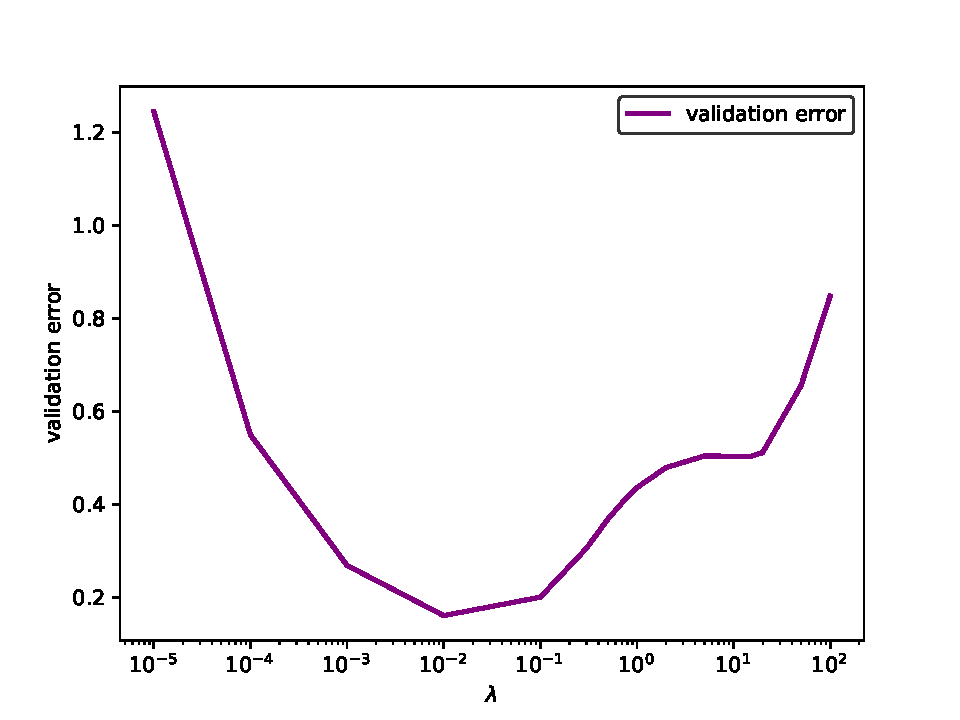
\includegraphics[width=0.5\linewidth]{tupian/validation.pdf}
    \caption{The validation error vs $\boldsymbol{\lambda}$}
    \label{val}
\end{figure}
As we can see from Figure \ref{val}, when $\lambda=10^{-2}$, we can get the smallest validation error.

\vspace{4pt}
\textbf{Subproblem (b2)}

We set $\lambda=$ 0.01, 0.1, 0.8 and 5 separately, and use the original training dataset to train the model. Then, we plot the fitted curve with 
different $\lambda$ as Figure \ref{lambda}.
\begin{figure}[H]
    \centering
    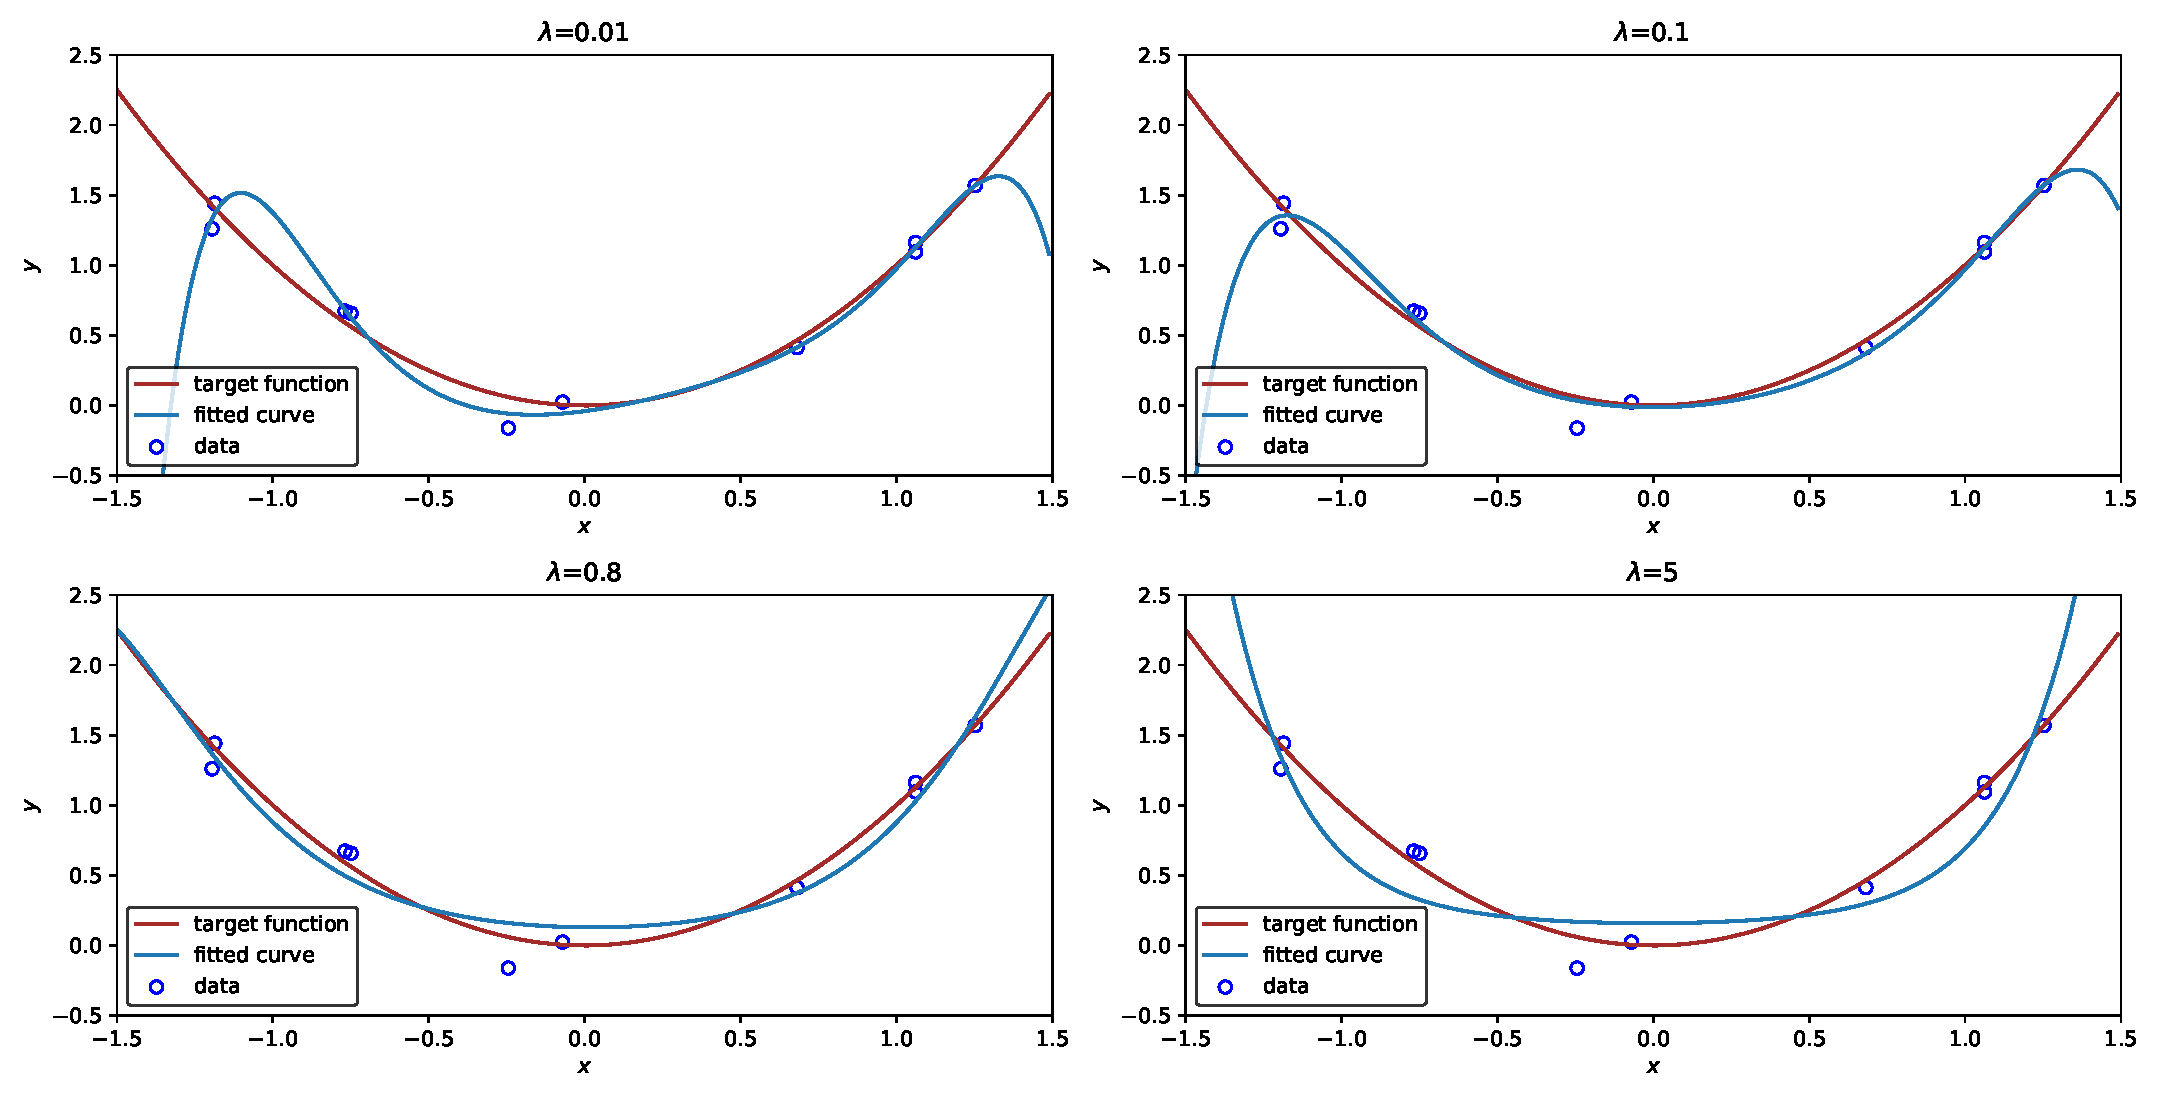
\includegraphics[width=0.9\linewidth]{tupian/lambda.pdf}
    \caption{The fitted curve with different $\boldsymbol{\lambda}$}
    \label{lambda}
\end{figure}
As we can see from Figure \ref{lambda}, when $\lambda=$0.01 and 0.1, it seems that the model is overfitted, and when $\lambda=5$, it seems that the model is underfitted. Finally, when $\lambda=$0.8, the model 
seems good and the fitted figure is close to the target function.

\vspace{4pt}
\textbf{Subproblem (b3)}

Using the test data set, we can calculate the test error $\|\boldsymbol{X}_{\text {test}} \widehat{\boldsymbol{\theta}}-\boldsymbol{y}_{\text {test}}\|_{2}$ of each of $\widehat{\boldsymbol{\theta}}$ obtained in (b2) as follow:
\begin{equation}
    \begin{split}
        &\lambda = 0.01: \quad\|\boldsymbol{X}_{\text {test}} \widehat{\boldsymbol{\theta}}-\boldsymbol{y}_{\text {test}}\|_{2}=12.46\\
        &\lambda = 0.1\,\,\, : \quad\|\boldsymbol{X}_{\text {test}} \widehat{\boldsymbol{\theta}}-\boldsymbol{y}_{\text {test}}\|_{2}=5.21\\
        &\lambda = 0.8\,\,\, : \quad\|\boldsymbol{X}_{\text {test}} \widehat{\boldsymbol{\theta}}-\boldsymbol{y}_{\text {test}}\|_{2}=0.42\\
        &\lambda = 5\,\,\,\,\,\,\,\, :\quad\|\boldsymbol{X}_{\text {test}} \widehat{\boldsymbol{\theta}}-\boldsymbol{y}_{\text {test}}\|_{2}=3.65
    \end{split}
\end{equation}

The Python code to solve Problem 3 is as follow
\begin{python}
import pandas as pd
import numpy as np
import matplotlib.pyplot as plt

#a1------------
data = pd.read_csv("Q3_training_data.csv", header=0, index_col=0)
x_train = np.array(data.iloc[0,:]).reshape(-1, 1)
y_train = np.array(data.iloc[1,:]).reshape(-1, 1)

#a2------------
x_sim = np.arange(-1.5, 1.5, 0.01)
y_sim = x_sim ** 2

plt.figure(1)
plt.plot(x_sim, y_sim, color="brown", label="target function")
plt.scatter(x_train, y_train, marker='o', c='', edgecolors='b', label="data")
plt.xlim(-1.5, 1.5)
plt.ylim(-0.5, 2.5)
plt.xlabel("$x$")
plt.ylabel("$y$")
plt.legend(loc="best", edgecolor="black")
plt.savefig("hw_tex/tupian/original.pdf")

order = 8
n_train = 10
x_train_new = np.ones(n_train).reshape(-1,1)
new_col = np.ones(n_train).reshape(-1,1)
for i in range(1,order+1):
    new_col = new_col * x_train
    x_train_new = np.hstack((x_train_new, new_col))
y_train_new = y_train
theta_hat = np.dot(np.dot(np.linalg.inv(np.dot(x_train_new.T, x_train_new)), x_train_new.T), y_train_new)

x_sim = np.arange(-1.5, 1.5, 0.01)
y_sim = np.zeros(len(x_sim))
for i in range(9):
    y_sim = y_sim + theta_hat[i] * (x_sim**i)

plt.plot(x_sim, y_sim, label="fitted curve")
plt.legend(loc="best", edgecolor="black")
plt.savefig("hw_tex/tupian/fitted.pdf")

#a3------------
data_test = pd.read_csv("Q3_test_data.csv", header=0, index_col=0)
x_test = np.array(data_test.iloc[0,:]).reshape(-1, 1)
y_test = np.array(data_test.iloc[1,:]).reshape(-1, 1)

n_test = 10
x_test_new = np.ones(n_test).reshape(-1,1)
new_col = np.ones(n_test).reshape(-1,1)
for i in range(1,order+1):
    new_col = new_col * x_test
    x_test_new = np.hstack((x_test_new, new_col))
y_test_new = y_test
test_error = np.linalg.norm(np.dot(x_test_new, theta_hat) - y_test_new, ord=2)
print("test error:", test_error)

#b1------------
lambda_candidate = [1e-5, 1e-4, 1e-3, 1e-2, 0.1, 0.3, 0.5, 0.8, 1, 2, 5, 10, 15, 20, 50, 100]
k = 5
s_size = n_train / k
error_list = []
for lambda_i in lambda_candidate:
    error = 0
    for val_i in range(k):
        x_val = x_train_new[[val_i*2, val_i*2+1], :]
        y_val = y_train_new[[val_i*2, val_i*2+1], :]
        x_train_val = np.vstack((x_train_new[0:val_i*2, :], x_train_new[val_i*2+2:, :]))
        y_train_val = np.vstack((y_train_new[0:val_i*2, :], y_train_new[val_i*2+2:, :]))
        I = np.identity(x_train_val.shape[1])
        theta_hat = np.dot(np.dot(np.linalg.inv(np.dot(x_train_val.T, x_train_val)+lambda_i*I), x_train_val.T), y_train_val)
        error  = error + np.linalg.norm(np.dot(x_val, theta_hat) - y_val, ord=2)

    error = error / k
    error_list.append(error)

plt.figure(2)
plt.semilogx(lambda_candidate, error_list, linewidth=2, color="purple", label="validation error")
plt.xlabel("$\lambda$")
plt.ylabel("validation error")
plt.legend(loc="best", edgecolor="black")
plt.savefig("hw_tex/tupian/validation.pdf")

#b2------------
lambda_candidate = [0.01, 0.1, 0.8, 5]
figure_num = 1
plt.figure(3, figsize=(20, 20))

test_error_list = []
for lambda_i in lambda_candidate:
    plt.subplot(2, 2, figure_num)
    figure_num = figure_num + 1
    
    x_sim = np.arange(-1.5, 1.5, 0.01)
    y_sim = x_sim ** 2
    plt.plot(x_sim, y_sim, color="brown", label="target function")
    plt.scatter(x_train, y_train, marker='o', c='', edgecolors='b', label="data")

    
    I = np.identity(x_train_new.shape[1])
    theta_hat = np.dot(np.dot(np.linalg.inv(np.dot(x_train_new.T, x_train_new)+lambda_i*I), x_train_new.T), y_train_new)
    x_sim = np.arange(-1.5, 1.5, 0.01)
    y_sim = np.zeros(len(x_sim))
    for i in range(9):
        y_sim = y_sim + theta_hat[i] * (x_sim**i)
    plt.plot(x_sim, y_sim, label="fitted curve")
    
    plt.xlim(-1.5, 1.5)
    plt.ylim(-0.5, 2.5)
    plt.xlabel("$x$")
    plt.ylabel("$y$")
    plt.title("$\lambda$={}".format(lambda_i))
    plt.legend(loc="lower left", edgecolor="black")
    plt.tight_layout()
    
    test_error = np.linalg.norm(np.dot(x_test_new, theta_hat) - y_test_new, ord=2)
    test_error_list.append(test_error)
    
plt.savefig("hw_tex/tupian/lambda.pdf")

#b3------------
print()
print("-"*20)
for i, test_error in enumerate(test_error_list):
    print("lambda={}, test error={}".format(lambda_candidate[i], test_error))
\end{python}
\end{homeworkProblem}
\begin{homeworkProblem}
The logistic regression developed in class is designated for Binary classification. How about when number of classes $K>2 ?$ The key idea is to assign each class $\ell=1, \ldots, K$ a weight vector $\boldsymbol{\theta}^{\ell} .$ Let $\boldsymbol{\Theta}=\left[\boldsymbol{\theta}^{1}, \ldots, \boldsymbol{\theta}^{K}\right] \in \mathbb{R}^{d \times K}$ and $\left\{\left(\boldsymbol{x}_{i}, y_{i}\right)\right\}_{i=1}^{n}$ be the training
data. The model for estimating the a-posteriori of $y_{i}$ is given by
$$
\operatorname{Pr}\left[y_{i}=\ell \mid \boldsymbol{\Theta}, \boldsymbol{x}_{i}\right]=\frac{\exp \left(\left\langle\boldsymbol{\theta}^{\ell}, \boldsymbol{x}_{i}\right\rangle\right)}{\sum_{j=1}^{K} \exp \left(\left\langle\boldsymbol{\theta}^{j}, \boldsymbol{x}_{i}\right\rangle\right)}
$$
It is clear that $\operatorname{Pr}\left[y_{i}=\ell \mid \boldsymbol{\Theta}, \boldsymbol{x}_{i}\right]$ sum to 1 over $\ell$. Using the reasoning of log-likelihood, we can formulate the learning problem as
\begin{equation}
    \label{eq10}
    \widehat{\boldsymbol{\Theta}}=\underset{\boldsymbol{\Theta} \in \mathbb{R}^{d \times K}}{\operatorname{argmin}}-\frac{1}{n} \sum_{i=1}^{n} \sum_{\ell=1}^{K} 1_{\left\{y_{i}=\ell\right\}} \log \left(\frac{\exp \left(\left\langle\boldsymbol{\theta}^{\ell}, \boldsymbol{x}_{i}\right\rangle\right)}{\sum_{j=1}^{K} \exp \left(\left\langle\boldsymbol{\theta}^{j}, \boldsymbol{x}_{i}\right\rangle\right)}\right)
\end{equation}
where $1_{\left\{y_{i}=\ell\right\}}$ is the indicator function defined as
$$
1_{\left\{y_{i}=\ell\right\}}=\left\{\begin{array}{ll}
1, & y_{i}=\ell \\
0, & O . W
\end{array}\right.
$$
\textbf{MNIST dataset} consists of 10 digits from 0 to 9 (i.e., $K=10$ ); see Figure \ref{MNIST}. Download the training and test dataset from blackboard. Each MNIST image is of dimension $28 \times 28 .$ We vectorize each image and this leads to $\boldsymbol{x}_{i} \in \mathbb{R}^{784}$ (i.e., $d=28 \times 28=784$ ). The training data consists of $n=2800$ digital images, while the test data consists of 200 images (each row represents one image).
\begin{figure}[htbp]
    \centering
    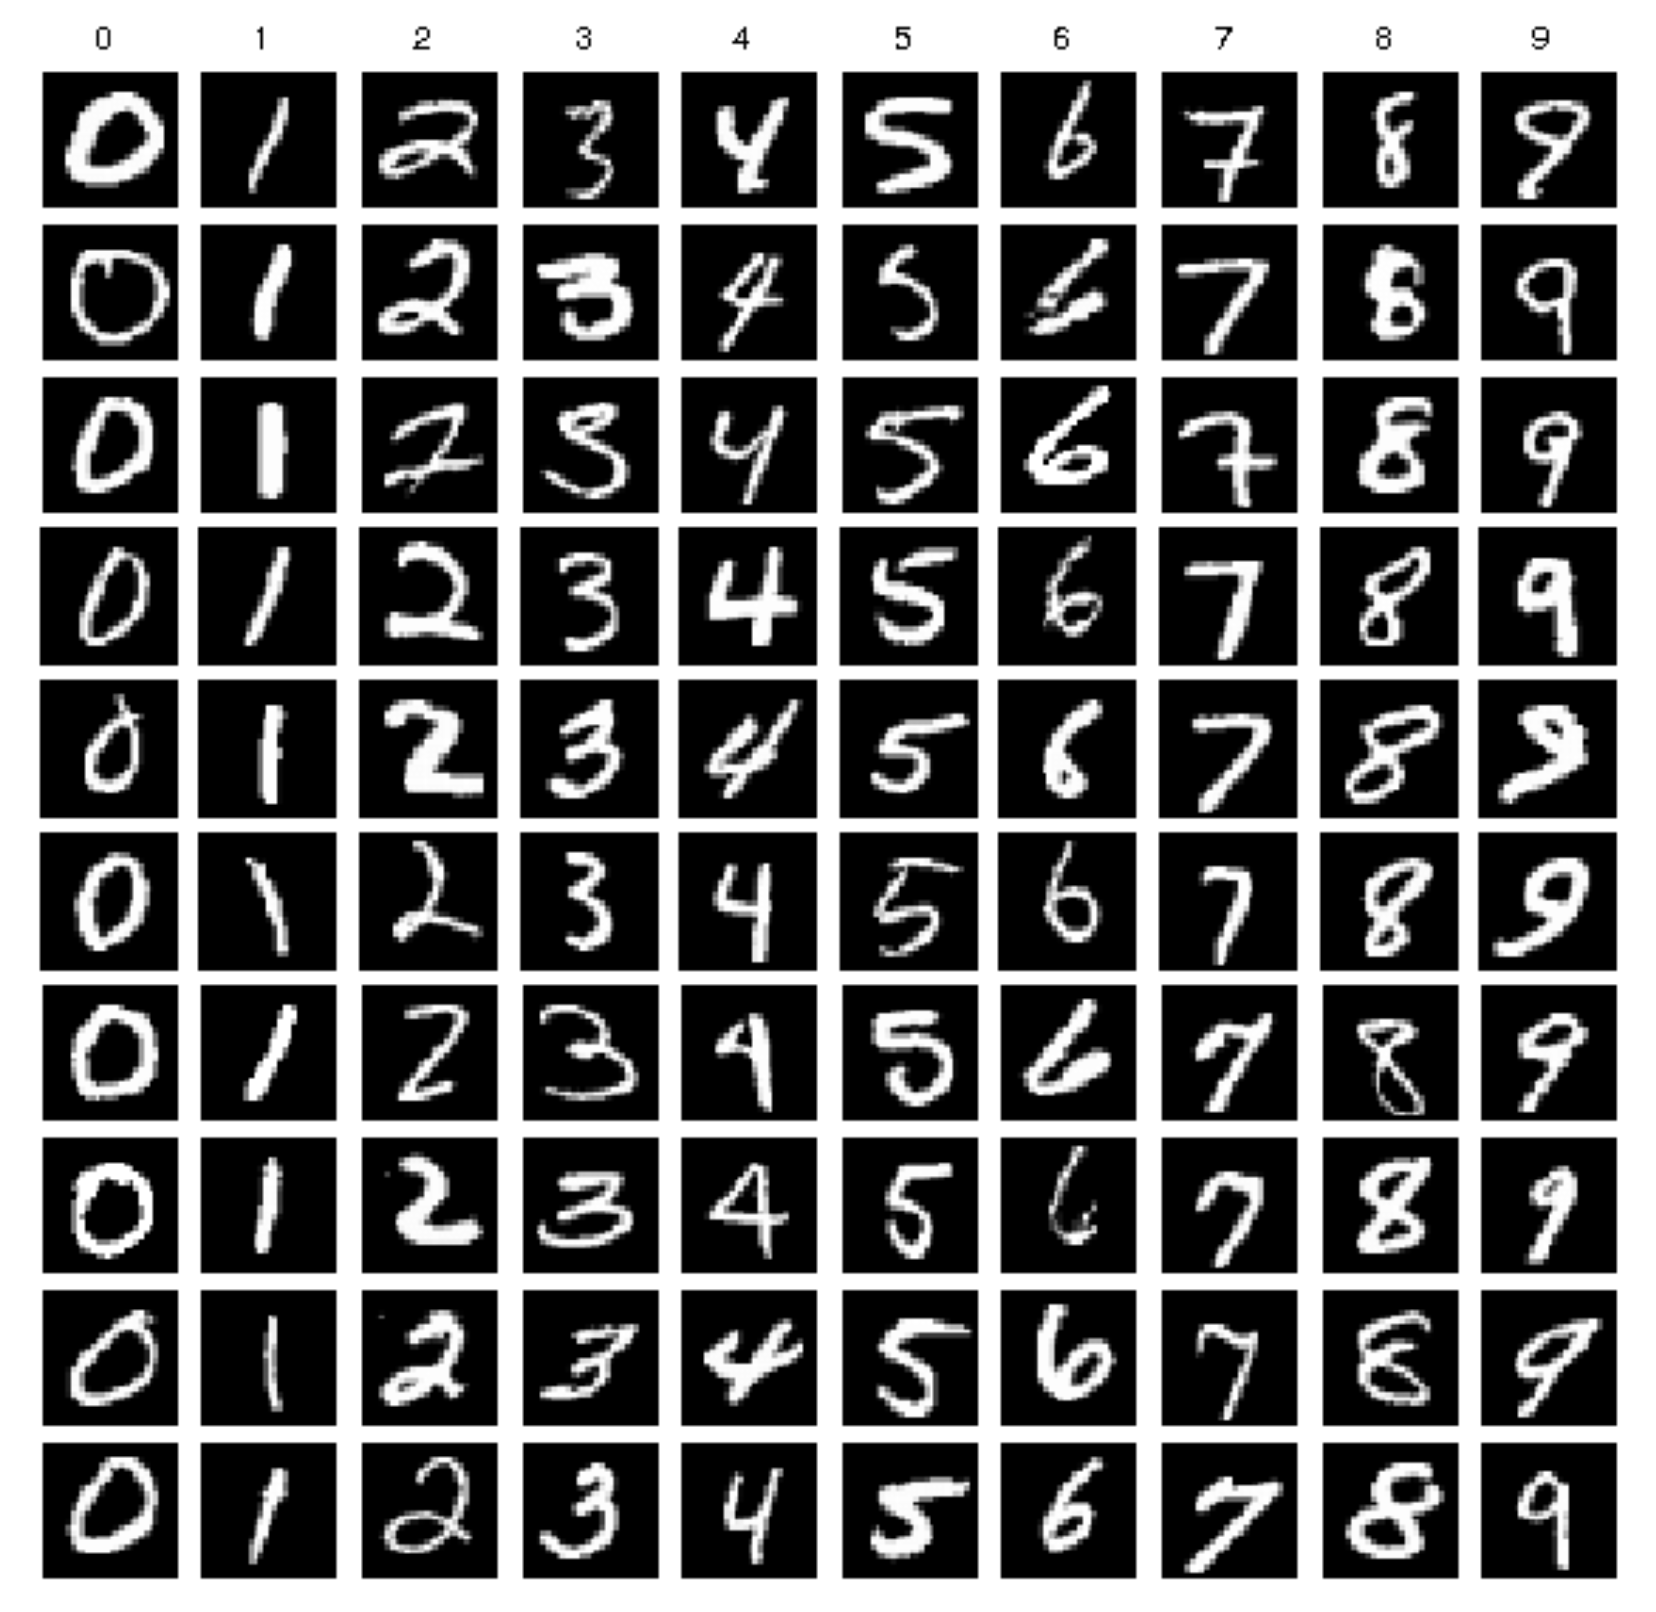
\includegraphics[width=0.4\linewidth]{tupian/MNIST}
    \caption{MNIST dataset}
    \label{MNIST}
\end{figure}

\textbf{Learning task}: Apply the multinomial logistic regression (\ref{eq10}) to this MNIST dataset and the settings are:
\begin{enumerate}[\quad$\bullet$]
    \item Using accelerated gradient descent algorithm.
    \item Set the stepsize to $\mu_{k}=\mu=0.01$.
    \item Start the algorithm at the origin.
    \item Set the total number of iterations to 500 .
    \item Plot the training accuracy versus iteration number.
    \item Plot the test accuracy versus iteration number.
\end{enumerate}

The classification rule is defined as the most natural one
$$\underset{j}{\operatorname{argmax}}\,\,\boldsymbol{e}_{j}^{\top} \widehat{\boldsymbol{\Theta}}^{\top} \boldsymbol{x}_{i}$$

\vspace{4pt}
\textbf{\large{Solution}}

The loss function is defined as follow
\begin{equation}
    \mathcal{L}\left(\boldsymbol{\Theta}\right)=-\frac{1}{n} \sum_{i=1}^{n} \sum_{\ell=1}^{K} 1_{\left\{y_{i}=\ell\right\}} \log \left(\frac{\exp \left(\left\langle\boldsymbol{\theta}^{\ell}, \boldsymbol{x}_{i}\right\rangle\right)}{\sum_{j=1}^{K} \exp \left(\left\langle\boldsymbol{\theta}^{j}, \boldsymbol{x}_{i}\right\rangle\right)}\right)
\end{equation}
Then, we can calculate the gradient due to the loss function in the matrix format as follow:
\begin{equation}
    \frac{\partial \mathcal{L}\left(\boldsymbol{\Theta}\right)}{\partial\boldsymbol{\Theta}}=\frac{1}{n}\cdot\boldsymbol{X}^{\top}\left(\boldsymbol{Z}-\boldsymbol{Y}\right)
\end{equation}
where
\begin{equation}
    \begin{split}
        \boldsymbol{X} &= 
        \begin{pmatrix}
            \cdots&\boldsymbol{x}_1&\cdots\\
            \cdots&\boldsymbol{x}_2&\cdots\\
            &\vdots&\\
            \cdots&\boldsymbol{x}_n&\cdots\\
        \end{pmatrix}\Longrightarrow \boldsymbol{X}\in\mathbb{R}^{n\times d}\\
        \\
        \boldsymbol{Y} &= 
        \begin{pmatrix}
            \cdots&\boldsymbol{y}_1&\cdots\\
            \cdots&\boldsymbol{y}_2&\cdots\\
            &\vdots&\\
            \cdots&\boldsymbol{y}_n&\cdots\\
        \end{pmatrix}\Longrightarrow \boldsymbol{Y}\in\mathbb{R}^{n\times K} \\
        &\left(\boldsymbol{y}_i \text{ is the one-hot presentation of labels}\right)\\
        \\
        \boldsymbol{Z}_{ij}&=\frac{\operatorname{exp}\left(\left\langle\boldsymbol{x}_i, \boldsymbol{\theta}^j\right\rangle\right)}{\sum_{k=1}^{K}\operatorname{exp}\left(\left\langle\boldsymbol{x}_i, \boldsymbol{\theta}^k\right\rangle\right)}\Longrightarrow \boldsymbol{Z}\in\mathbb{R}^{n\times K}
    \end{split}
\end{equation}
By using Python, we implement the accelerated gradient descent algorithm with $\mu_{k}=\mu=0.01$, and set the initial point as origin. Besides, we fixed the iteration number to be 500. 
The figure of training accuracy versus iteration number and test accuracy versus iteration number is showed as Figure \ref{accuracy}.
\begin{figure}[H]
    \centering
    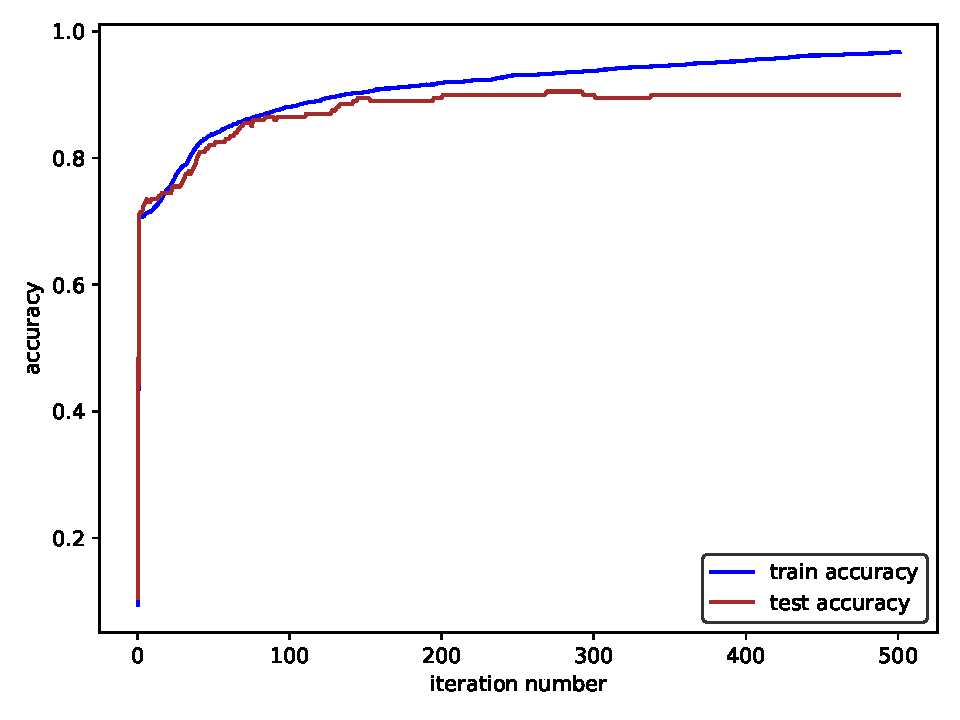
\includegraphics[width=0.5\linewidth]{tupian/accuracy}
    \caption{The training accuracy and test accuracy curve}
    \label{accuracy}
\end{figure}

As we can see from Figure \ref{accuracy}, the training accuracy and test accuracy increase very fast at the beginning.
Then consinuously increases with the increase of iteration number, but the speed is becoming slower. Finally, the train accuracy will 
reach 96.75\% at iteration 500, and the test accuracy will be constant when it reaches to 90\%.

The Python code to solve Problem 4 is as follow
\begin{python}
import pandas as pd
import numpy as np
import matplotlib.pyplot as plt

#training data
training_data = pd.read_csv("Q4_MNIST_train.csv", header=0, index_col=0)
x = np.array(training_data.iloc[:, 0])
y = np.array(training_data.iloc[:, 1])
K = 10 #number of class 

for i in range(len(x)):
    x_i = x[i][1:-1].split(',')
    for j in range(len(x_i)):
        x_i[j] = float(x_i[j])
    x_i = np.array(x_i).reshape(1,-1)
    if i==0:
        X_train = x_i
    else:
        X_train = np.vstack((X_train, x_i))

for i in range(len(y)):
    l = int(y[i][1:-1])
    y_i = np.zeros(K)
    y_i[l-1] = 1
    if i == 0:
        y_train = y_i
    else:
        y_train = np.vstack((y_train, y_i))

n = X_train.shape[0]
dim = X_train.shape[1]

#testing data
test_data = pd.read_csv("Q4_MNIST_test.csv", header=0, index_col=0)
x = np.array(test_data.iloc[:, 0])
y = np.array(test_data.iloc[:, 1])

for i in range(len(x)):
    x_i = x[i][1:-1].split(',')
    for j in range(len(x_i)):
        x_i[j] = float(x_i[j])
    x_i = np.array(x_i).reshape(1,-1)
    if i==0:
        X_test = x_i
    else:
        X_test = np.vstack((X_test, x_i))

for i in range(len(y)):
    l = int(y[i][1:-1])
    y_i = np.zeros(K)
    y_i[l-1] = 1
    if i == 0:
        y_test = y_i
    else:
        y_test = np.vstack((y_test, y_i))

#calculate gradient
def cal_grad(theta):
    Z = np.dot(X_train, theta)
    exp_Z = np.exp(Z)
    sum_Z = np.sum(exp_Z, axis=1).reshape(-1, 1)
    vector_Z = exp_Z / sum_Z
    
    grad = np.dot(X_train.T, vector_Z-y_train)
    grad = grad / n
    return grad

def cal_accuracy(theta, X, y):
    total_num = X.shape[0]
    y_predict = np.argmax(np.dot(X, theta), axis=1)
    y = np.argmax(y, axis=1)
    correct_num = np.sum(y_predict == y)
    return correct_num / total_num

def plot_convergence(train_accuracy, test_accuracy):
    iteration_num = len(train_accuracy)
    iterate = range(iteration_num)
    
    plt.figure(1)
    plt.plot(iterate, train_accuracy, color="blue", label="train accuracy")
    plt.plot(iterate, test_accuracy, color="brown", label="test accuracy")
    plt.xlabel("iteration number")
    plt.ylabel("accuracy")
    plt.legend(loc="best", edgecolor="black")
    plt.tight_layout()
    plt.savefig("hw_tex/tupian/accuracy.pdf")
    
def AGD(initial):
    
    mu = 0.01 # step size
    theta_minus = initial
    theta_k = initial
    
    num_iteration = 0
    
    train_accuracy = []
    test_accuracy = []
    
    train_accuracy.append(cal_accuracy(theta_k, X_train, y_train))
    test_accuracy.append(cal_accuracy(theta_k, X_test, y_test))
    while num_iteration <= 500:
        
        beta_k = (num_iteration-1)/(num_iteration+2)
        w = theta_k + beta_k * (theta_k - theta_minus)
        
        theta_minus = theta_k
        theta_k = w - mu * cal_grad(w)
        
        train_accuracy.append(cal_accuracy(theta_k, X_train, y_train))
        test_accuracy.append(cal_accuracy(theta_k, X_test, y_test))
        
        num_iteration  = num_iteration + 1
        
    plot_convergence(train_accuracy, test_accuracy)
    print("train accuracy at the last step:", train_accuracy[-1])
    print("test accuracy at the last step:", test_accuracy[-1])
theta_initial = np.zeros((dim, K))
AGD(theta_initial)    
\end{python}
\end{homeworkProblem}
\end{document}
